\documentclass[12pt]{extarticle}
\usepackage{array}
\usepackage[T1]{fontenc}
\usepackage[Russian]{babel}
\usepackage{booktabs}
\usepackage{graphicx}
\usepackage{spreadtab}
\usepackage{numprint}
\usepackage[margin=3cm]{geometry}
\usepackage{float}
\usepackage{xfp}
\usepackage{amsmath}   
\begin{document}
\author{Осипов Александр Б06-604}
\title{Лабораторная работа 1.1.1. Определение систематических и случайных погрешностей при измерении удельного сопротивления нихромовой проволки}
\maketitle
\section{Цель}

Измерить удельное сопротивлене проволки и вычислить систематические и случаные погрешности
при использовании таких измерительных приборов, как линейка,
штангенциркуль, микрометр, амперметр, вольтметр и мост постоянного тока.

\section{Оборудование} 

Вольметр, амперметр, штангенциркуль, микрометр, линейка
проволка из нихрома, источник ЭДС, мост постоянного тока.

\section {Теоретическая часть}

Для вычисления удельного сопротивления проволки будет использовать следующая формула:
$$
\rho = \frac{R \pi d^2}{4l}
$$
где,

R - сопротивление проволки;

l - длина проволки;

d - диаметр проволки;

\vspace{0.5cm} 
Для расчёта диаметра проволки испольуется штангенциркуль и микрометр.

\newpage 
Сопротивление измеряется с использованием одной из следующих электрических схем:

\begin{center}
  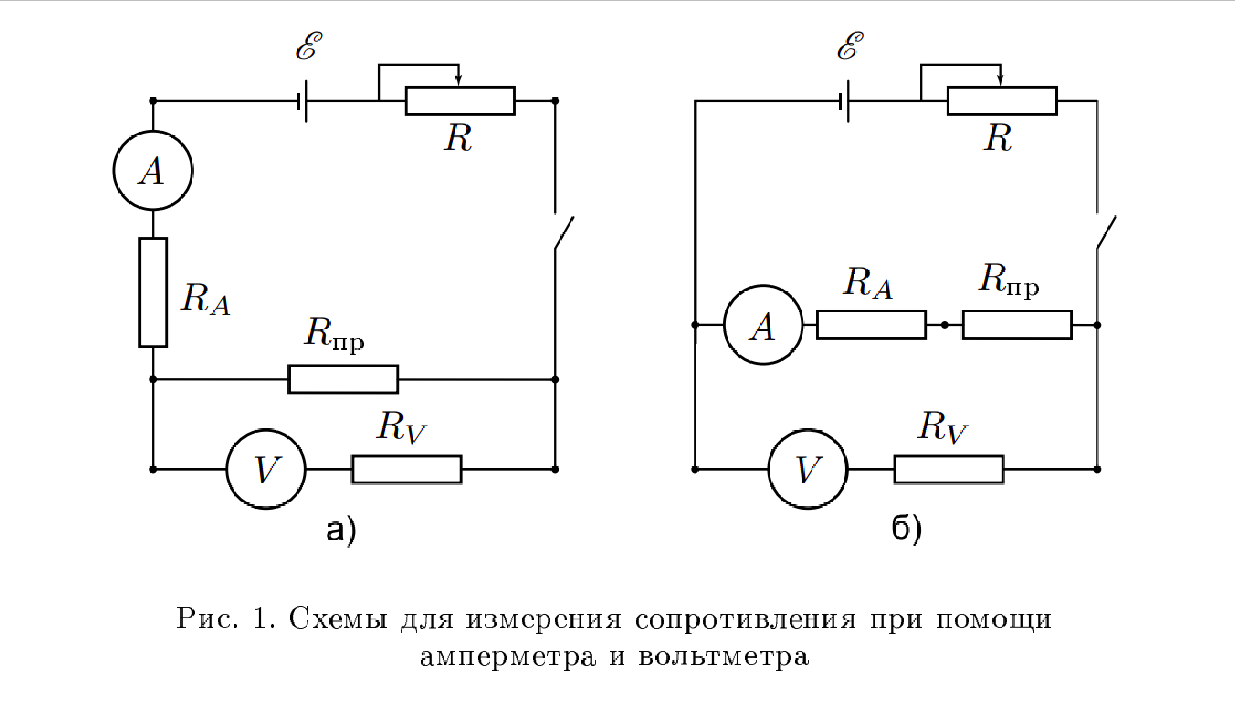
\includegraphics[scale=0.6]{assets/lab_1_1_1_scheme.png}
\end{center}

Учитвая, что приборы имеют некоторое сопротивление, истинные значения R можно расчитать
в соответстии со следующими формулами:

$$
R = R_1(1 + \frac{R_1}{R_V})
$$
для схемы 1, где:

$R_1$ - сопротивление проволки, расчитанное из показаний амперметра и вольтметра при измерениис помощью схемы 1;

$R_V$ - сопротивление вольтметра;

$$
R = R_2(1-\frac{R_A}{R_2})
$$
для схемы 2, где:

$R_2$ - сопротивление проволки, расчитанное из показаний амперметра и вольтметра при измерениис помощью схемы 1;

$R_A$ - сопротивление амперметра.

\newpage 
\section{Ход работы}
\vspace{0.5cm}

Для расчётов, проведенных в Jupyter Notebook используется ссылка (python)

\vspace{0.5cm} 

d1 - измерения микрометром

\noindent d2 - измерения штангенциркулем
\vspace{\baselineskip}

\textbf{\large Таблица 1 - результаты измерения диаметра проволки}
 
\vspace{0.5cm}

\begin{spreadtab}{{tabular}{c|c|c|c|c|c|c|c|c|c|c|c}}
     &1&2&3&4&5&6&7&8&9&10&@\text{среднее} \\ 
    @d1, mm & 0.34 & 0.35 & 0.36 & 0.36 & 0.37 & 0.36 & 0.36 & 0.36 & 0.36 &0.36 & sum(b2:k2)/10 \\
    @d2, mm & 0.4 & 0.4 & 0.4 & 0.4 & 0.4 & 0.4 & 0.4 & 0.4 & 0.4 & 0.4 \\
\end{spreadtab}

\vspace{0.5cm}

\vspace{0.5cm}
Результаты измерения штангенциркулем:

$ d = (0.4 \pm 0.1)$

Результаты измерения микрометром:

$\sigma_{\text{сл.}} = 0.002 \text{мм}$  (python)

$\sigma_{\text{сист.}} = 0.01 \text{мм}$

$\sigma = (\sigma_{\text{сист.}}^2 + \sigma_{\text{сл.}}^2)^{(1/2)} = \fpeval{round((0.01^2 + 0.002^2)^{(1/2)}, 3)} \text{мм}$

$d = 0.358 \pm 0.01 \text{мм}$
\vspace{0.5cm}

\textbf{\large Таблица 2 - Основные характеристики приборов}

\begin{tabular}{ccc}
     & Вольтметр & Миллиамперметр\\
    Система & магнитоэлектрическая& электронная\\
    Класс точности & 0.5& -\\
    Цена деления & 5мВ/дел. & - \\
    Абс. погрешность: & 1.875 мВ & 0.01 мА \\
    Сист. погрешность: & 0.9375 мВ & 0.005 мА \\
    Внутреннее сопротивление & 5 кОм & 1.2 Ом \\
\end{tabular}

\vspace{5mm}

Оценка ошибки при измерении схемой а и б:
 
$ \text{a: } R/R_V = \fpeval{5/5000} $

$ \text{б: } R_{А}/R = \fpeval{1.2/5} $

Следовательно, для эксперимента выбрана схема (а).

\newpage

\textbf{\large Таблица 3 - Показания вольтметра и амперметра}

\begin{table}[H]
    \resizebox{\textwidth}{!}{
        \begin{tabular}{c|c|c|c|c|c|c|c|c|c|c|c|c}
            \multicolumn{4}{c}{l = 20 см} |& \multicolumn{4}{c}{l = 30 см} |& \multicolumn{4}{c}{l = 50 см}\\ 
            & V,дел & I,дел & V,мВ & I, мА | & V,дел & I,дел & V,мВ & I, мА | & V,дел & I,дел & V,мВ & I, мА\\
            \toprule 
            1 & 147 & 358.8 & 735& 358.8 |  & 149 & 245.7 & 745 & 245.7 | & 150 & 148.2 & 750 & 148.2\\
            \midrule
            2 & 136 & 333.4 & 680 & 333.4 | & 123 & 203.0 & 615 & 203.0 | & 131 & 129.9 & 655 & 129.9\\
            \midrule
            3 & 117 & 286.2 & 585 & 286.2 | & 101 & 174.9 & 505 & 174.9 | & 124 & 122.2 & 620 & 122.2\\
            \midrule
            4 & 98 & 239.2 & 490 & 239.5 | & 95 & 156.7 & 475 & 156.7 | & 109 & 107.9 & 545 & 107.9\\
            \midrule
            5 & 79 & 191.5 & 395 & 191.5 | & 83 & 136.7 & 415 & 136.7 | & 95 & 094.2 &  475 & 094.2\\
            \midrule
            6 & 67 & 164.1 & 335 & 164.1 | & 66 & 109.0 & 330 & 109.0 | & 87 & 085.7 & 435 & 085.7\\
            \midrule
            7 & 59 & 131.5 &  295 & 131.5 | & 50 & 083.3 & 250 & 083.3 | & 82 & 081.0 & 410 & 081.0\\
            \midrule
            8 & 43 & 106.3 & 215 & 106.3 | & 45 & 075.2 & 225 & 075.2 | & 75 & 074.6 & 375 & 074.6\\
            \midrule
            9 & 30 & 073.6 & 150 & 073.6 | & 42 & 069.6 & 210 & 069.9 | & 69 & 068.4 & 345 & 068.4\\
            \midrule
            10 & 26 & 065.3 & 130 & 065.3 | & 39 & 064.1 & 195 & 064.1 | & 62 & 061.7 & 310 & 061.7\\
            \midrule
        \end{tabular}
    }
\end{table}
\vspace{5mm}

Из графика (python) проверяем, что нет различия между значениями, полученными при возрастании 
и при уменьшении тока:

\begin{center}
  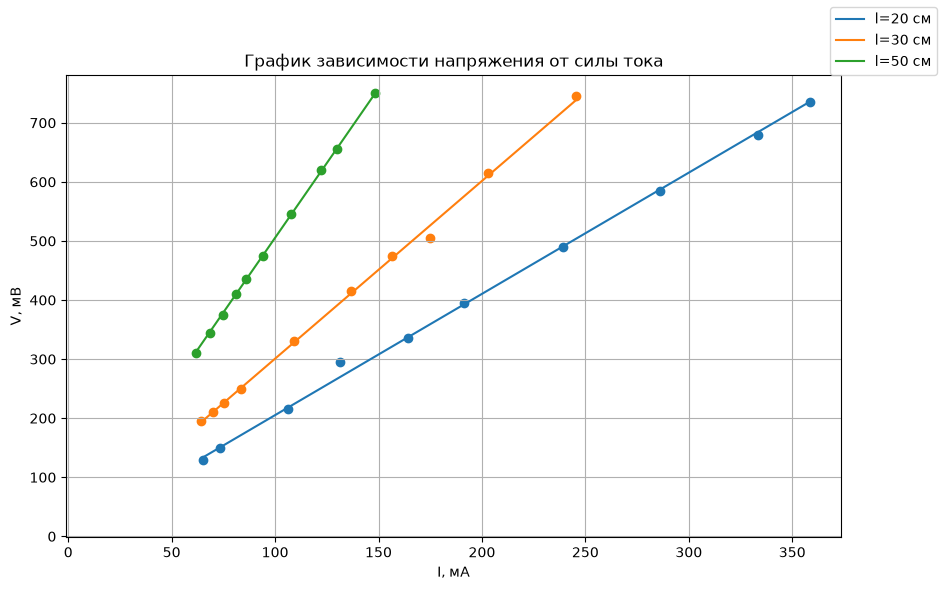
\includegraphics[scale=0.7]{assets/plot_lab_111.png}
\end{center}

\newpage 

\textbf{\large Таблица 4 - Результаты измерения сопротивления проволки} (python)

\vspace{5mm}

\begin{tabular}{cccc}
     & l = 20 мм& l = 30см & l = 50 см\\
    R(по Р4833) & 2.1797 & 3.1669 & 5.2225\\
    $R_{\text{ср}}$&2.052 & 3.008 & 5.054\\
    $\sigma{\text{сл}}$& 0.012 & 0.016 & 0.005\\
    $\sigma{\text{сист}}$& 0.003 & 0.004 & 0.006\\
    $\sigma$& 0.012 & 0.016 & 0.008\\

\end{tabular}

\textbf{\large Таблица 5 - Результаты расчета удельного сопротивления проволки}

\vspace{5mm}

\begin{tabular}{ccc}
    l, см & $\rho$, $10^{-4}$ Ом*см & $\sigma_{\rho}$, $10^{-6}$ Ом*см\\
    20 см & 1.03 & 0.03\\
    30 см & 1.01 & 0.03\\
    50 см & 1.02 & 0.03\\

\end{tabular}

\section{Вывод:}

С помощью данного эксперимента было измерено удельное сопротивление нихромовой проволки.
Результат:

$$\rho = 1.02 \pm 0.03 \text{ Ом * см}$$ 

\end{document}